\section{Theoretical Analysis}
\label{sec:theory}

% This section provides a theoretical perspective that explains the empirical findings in Section~\ref{sec:motivation}.
% We analyze why different actions in deep research agents exhibit fundamentally different sensitivities to explicit reasoning, and why this leads to distinct optimal speculation pathways.

% Our central claim is that Search and Visit actions differ in their intrinsic decision uncertainty.
% Explicit reasoning reduces uncertainty by introducing intermediate structure, but its benefit depends on the property of the action type.
% We formalize this intuition using an entropy-based analysis of action policies and show that Search actions admit significantly larger uncertainty reduction from reasoning than Visit actions.
% This provides a theoretical explanation for the System~2 vs.\ System~1 dichotomy observed empirically.

This section provides a theoretical explanation for the empirical observations in Section~\ref{sec:motivation}.
We analyze why different actions exhibit distinct sensitivities to explicit reasoning, leading to different optimal speculation strategies.

Our central claim is that Search and Visit actions differ in intrinsic decision uncertainty.
% While explicit reasoning reduces uncertainty by introducing intermediate structure, its effectiveness depends on the action type.
We formalize this intuition via an entropy-based analysis of action policies and show that Search actions benefit significantly more from reasoning-induced uncertainty reduction than Visit actions, explaining the empirically observed System~2 versus System~1 dichotomy.


\subsection{Preliminaries: Action Policies and Entropy}

At each step, an agent observes a state $s$ from the accumulated context and then samples an action $a$ 
from a policy $\pi(\cdot \mid s)$.
We denote the action spaces corresponding to Search and Visit by $\mathcal{A}_{\textsc{search}}$ and $\mathcal{A}_{\textsc{visit}}$, respectively.



A natural measure of decision uncertainty is the conditional entropy of the action policy:
\begin{equation}
H(\pi(\cdot \mid s)) \;=\; -\sum_{a \in \mathcal{A}} \pi(a \mid s)\log \pi(a \mid s).
\label{eq:policy_entropy}
\end{equation}
Lower entropy indicates a more confident and concentrated decision, whereas higher entropy reflects ambiguity among many plausible actions.

In deep research agents, however, actions are expressed as open-ended language strings (e.g., search queries or extraction instructions), rendering exact computation of~\eqref{eq:policy_entropy} intractable.
We therefore adopt a token-level proxy based on the negative log-likelihood of the realized action.
Specifically, for an action represented as a token sequence $a=(t_1,\ldots,t_n)$, we define the mean token-level entropy proxy:
\begin{equation}
\bar{H}(a \mid s) \;=\; \frac{1}{n}\sum_{i=1}^n \left(-\log p(t_i \mid s, t_{<i})\right),
\label{eq:token_entropy_proxy}
\end{equation}
where smaller $\bar{H}(a \mid s)$ (i.e., higher average token log probability) indicates lower decision uncertainty.


\subsection{Intrinsic Entropy Gap Between Search and Visit}

We first examine the baseline uncertainty of different actions when generated \emph{without} explicit reasoning.
Intuitively, Search actions map a broad and ambiguous intent to a concrete query, for which many formulations may be reasonable.
In contrast, Visit operates on retrieved candidates and localized content, significantly constraining the decision space.

\begin{figure}
    \centering
    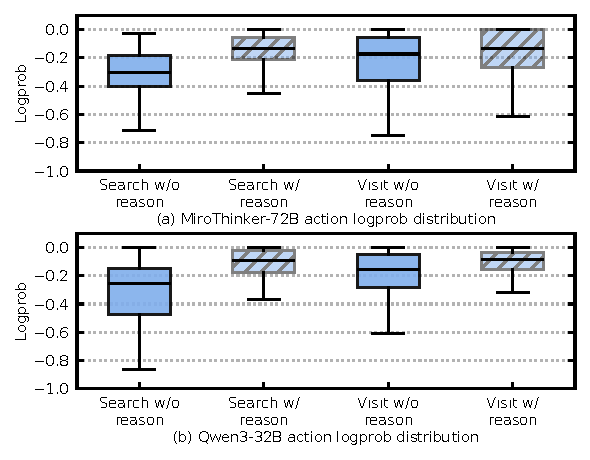
\includegraphics[width=\linewidth]{figs/logprob.pdf}
    \caption{Action log probability distributions with and without reasoning. 
    % We report the distribution of per-action mean token log probabilities for Search and Visit under two inference modes.
    A higher log probability indicates lower uncertainty.
    Without reasoning (dark blue color), Search actions exhibit lower log probabilities than Visit actions, indicating higher baseline decision uncertainty. 
    When reasoning is incorporated (light blue color with hatching), both action types see increased log probabilities, but the increase is significantly larger for Search actions, reflecting a greater reduction in uncertainty due to reasoning.}
    \label{fig:entropy_boxplot}
\end{figure}

This intuition is reflected in the following inequality:
\begin{equation}
    \mathbb{E}[\bar H(a\mid s)\mid a\in\mathcal{A}_{\textsc{search}}]
\;>\;
\mathbb{E}[\bar H(a\mid s)\mid a\in\mathcal{A}_{\textsc{visit}}].
\end{equation}
That is, under identical inference settings, Search actions exhibit higher average uncertainty than Visit actions.
Figure~\ref{fig:entropy_boxplot} visualizes this gap.
Each boxplot shows the distribution of mean token log probabilities for Search and Visit actions. 
When generated without reasoning, 
Search consistently exhibits lower log probabilities (higher $\bar{H}$) than Visit, suggesting less confident action distribution.


\subsection{Why Reasoning Helps: Entropy Reduction via Intermediate Structure}

We model explicit reasoning as the introduction of an intermediate latent variable $z$, corresponding to a reasoning trace that refines the decision context before the final action is generated.
This transforms the direct mapping $\pi(a \mid s)$ into a two-stage generation process:
\begin{equation}
\pi(a \mid s) \;=\; \sum_{z} \pi(z \mid s)\,\pi(a \mid s, z),
\label{eq:latent_factorization}
\end{equation}
where the final action is conditioned not only on the original state $s$, but also on the intermediate reasoning state $z$.
By a standard information-theoretic property~\cite{cover1999elements}, conditioning cannot increase entropy.
Formally,
\begin{equation}
\mathbb{E}_{z\sim \pi(\cdot\mid s)}\!\left[ H(\pi(\cdot \mid s, z)) \right] \;\le\; H(\pi(\cdot \mid s)).
\label{eq:entropy_reduction}
\end{equation}
Thus, access to a reasoning trace reduces action uncertainty and increases the likelihood of the realized action.


As shown in Figure~\ref{fig:entropy_boxplot}, incorporating reasoning consistently increases log probabilities, corresponding to a reduction in action-level uncertainty.
This reduction is most pronounced when the target decision relies on non-local associations that are not directly specified in the immediate input~\cite{prystawski2023think}.
Therefore, for Search, reasoning decomposes a global, underspecified mapping into a sequence of more localized sub-decisions, yielding a large reduction in uncertainty.
In contrast, Visit actions already exhibit low baseline entropy due to strong grounding in retrieved content.
Therefore, conditioning on an reasoning trace yields only a marginal additional reduction in uncertainty.


Taken together, this analysis explains why Search aligns more closely with \emph{System~2} behavior, while Visit is closer to \emph{System~1} behavior in deep research agents.



% this analysis explains the asymmetric benefit of reasoning observed in Section~\ref{sec:motivation}.
% Search actions operate in a high-entropy regime, where explicit reasoning plays a critical role in reducing uncertainty and improving decision quality.
% Visit actions, by contrast, operate in a low-entropy regime, where direct inference with sufficient model capacity is more helpful.
% This distinction closely mirrors the System~2 vs.\ System~1 dichotomy from dual-process theory.





\iffalse

Initial draft:

This section analyzes the underlying factors that differentiate \textit{System~2} and \textit{System~1} actions in deep research agents.
Specifically, we study why some actions benefit substantially from additional reasoning to reduce decision uncertainty, whereas others can be reliably produced by directly operating on concrete inputs.
To this end, we conduct an entropy-based analysis that quantifies action-level uncertainty and connects it to different inference pathways.

\subsection{Preliminaries: Action Policy and Entropy}
At each step, an agent observes a state $s$ (previous context) and samples an action $a \sim \pi(\cdot \mid s)$.
We denote the corresponding action sets of \textsc{Search} and \textsc{Visit} by $\mathcal{A}_{\textsc{search}}$ and $\mathcal{A}_{\textsc{visit}}$, respectively.

A natural measure of decision uncertainty is the conditional entropy of the action policy:
\begin{equation}
H(\pi(\cdot \mid s)) \;=\; -\sum_{a \in \mathcal{A}} \pi(a \mid s)\log \pi(a \mid s).
\label{eq:policy_entropy}
\end{equation}
However, in deep research agents, actions are emitted as open-ended natural-language strings (e.g., queries and URLs), making $H(\pi(\cdot \mid s))$ intractable to compute exactly.
We therefore use the per-token negative log-likelihood of the realized action as a tractable uncertainty proxy.
Concretely, for an action rendered as tokens $a = (t_1,\ldots,t_n)$, we compute
\begin{equation}
\bar{H}(a \mid s) \;=\; \frac{1}{n}\sum_{i=1}^n \left(-\log p(t_i \mid s, t_{<i})\right),
\label{eq:token_entropy_proxy}
\end{equation}
where a smaller $\bar{H}(a\mid s)$ (equivalently, a higher mean token log probability) indicates lower decision uncertainty.


\subsection{Entropy Gap Between \textsc{Search} and \textsc{Visit}}

We then compare action uncertainty under inference with and without explicit reasoning.
Intuitively, \textsc{Search} transforms a broad and ambiguous intent into a concise query, offering many plausible outputs. In contrast, \textsc{Visit} operates on returned content and often involves simpler decisions like selecting or extracting information, which inherently reduces ambiguity.


Our empirical findings confirm this intuition: in the absence of explicit reasoning,
\begin{equation}
    \mathbb{E}[\bar H(a\mid s)\mid a\in\mathcal{A}_{\textsc{search}}]
\;>\;
\mathbb{E}[\bar H(a\mid s)\mid a\in\mathcal{A}_{\textsc{visit}}].
\end{equation}
demonstrating an intrinsic entropy gap between \textsc{Search} and \textsc{Visit} actions.

\begin{figure}
    \centering
    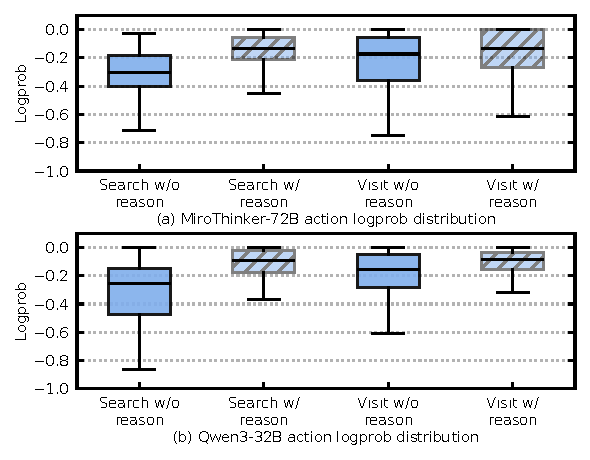
\includegraphics[width=\linewidth]{figs/logprob.pdf}
    \caption{Action log probability distributions with and without reasoning. We report the distribution of per action mean token log probabilities for \textsc{Search} and \textsc{Visit} under two inference modes. Results are shown for (a) MiroThinker-72B and (b) Qwen3-32B. \textsc{Visit} actions exhibit higher log probabilities even when generated without reasoning, suggesting lower baseline decision uncertainty.
    Consequently, the increase in action log probability brought by reasoning is substantially larger for \textsc{Search} than for \textsc{Visit}.}
    \label{fig:entropy_boxplot}
\end{figure}

Figure~\ref{fig:entropy_boxplot} visualizes this baseline difference.
Each boxplot shows the distribution of mean token log probabilities for \textsc{Search} and \textsc{Visit} actions when generated without reasoning.
Compared to \textsc{Visit}, \textsc{Search} consistently exhibits lower log probabilities (higher $\bar{H}$), suggesting larger decision uncertainty.

\subsection{Why Reasoning Helps: Entropy Reduction via Intermediate Structure}

We model explicit reasoning as introducing an intermediate latent variable $z$ (a reasoning trace) that refines the decision context before committing to the final action.
This transforms the direct mapping $\pi(a \mid s)$ into a two-stage generation process:
\begin{equation}
\pi(a \mid s) \;=\; \sum_{z} \pi(z \mid s)\,\pi(a \mid s, z),
\label{eq:latent_factorization}
\end{equation}
which can be viewed as marginalizing over possible reasoning traces.
By the standard property that conditioning cannot increase entropy, we have
\begin{equation}
\mathbb{E}_{z\sim \pi(\cdot\mid s)}\!\left[ H(\pi(\cdot \mid s, z)) \right] \;\le\; H(\pi(\cdot \mid s)),
\label{eq:entropy_reduction}
\end{equation}
suggesting that access to the latent trace $z$ reduces uncertainty and increases the likelihood of the final action.


As shown in Figure~\ref{fig:entropy_boxplot}, incorporating reasoning consistently increases action log probabilities, corresponding to a reduction in action-level uncertainty.
This reduction is most pronounced when the target decision relies on non-local associations that are not directly specified in the immediate input~\cite{prystawski2023think}.
In our setting, \textsc{Search} requires translating an abstract research goal into a concrete query, where many alternatives are plausible and the direct distribution is diffuse.
Reasoning introduces intermediate structure that decomposes this mapping into more localized sub-decisions, concentrating probability mass and yielding a larger reduction in uncertainty.

By contrast, \textsc{Visit} actions are more directly grounded in retrieved candidates and content, leading to a sharper action distribution even under non-reasoning inference.
As a result, additional reasoning yields a smaller marginal reduction in uncertainty.
Overall, these findings explain why \textsc{Search} aligns more closely with \emph{System~2} behavior, while \textsc{Visit} is closer to \emph{System~1} behavior in deep research agents.

\fi


% Putting the above together, we interpret \textsc{Search} as a \textit{System~2}-like action: it starts from a higher-entropy decision space and thus benefits more from explicit reasoning that reduces uncertainty before action emission.
% In contrast, \textsc{Visit} is \textit{System~1} action: its action entropy is naturally low, so additional reasoning yields limited marginal gain; performance instead depends on the model's parametric capacity to rapidly recognize and extract useful information from concrete inputs.

